\tikzstyle{process} = [rectangle, minimum width=1cm, minimum height=1cm, text centered, text width=1cm, draw=black, fill=blue!10]

\tikzstyle{arrow} = [thick,->,>=stealth]

% --- %

\resizebox{8cm}{!} {%
  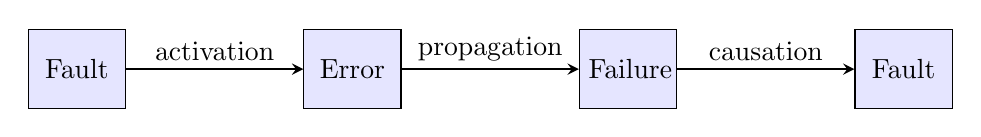
\begin{tikzpicture}[align=center, node distance=1cm]

  \node (f1) [process] {Fault};
  \node (f2) [process, right of=f1, xshift=2.5cm] {Error};
  \node (f3) [process, right of=f2, xshift=2.5cm] {Failure};
  \node (f4) [process, right of=f3, xshift=2.5cm] {Fault};

  % --- %

  \draw [arrow] (f1) -- node[anchor=south, yshift=-0.025cm] {activation} (f2);
  \draw [arrow] (f2) -- node[anchor=south, yshift=-0.025cm] {propagation} (f3);
  \draw [arrow] (f3) -- node[anchor=south, yshift=-0.025cm] {causation} (f4);

  \end{tikzpicture}
}
